\def\pgfsysdriver{pgfsys-dvisvgm.def}
% flashcards-title: Observed life-process criteria in three cases
% flashcards-desc: A four-column matrix uses filled circles for observed processes and open circles for processes not observed. Case A has four filled circles, Case B two, and Case C one.
\documentclass[tikz,border=6pt]{standalone}
\usetikzlibrary{arrows.meta,calc,fit,positioning,shapes.geometric}

\definecolor{fcink}{HTML}{17212B}
\definecolor{fcblue}{HTML}{1D5D8C}
\definecolor{fcgreen}{HTML}{2D6A4F}
\definecolor{fcorange}{HTML}{A44A1F}
\definecolor{fcpale}{HTML}{F4F7F9}
\definecolor{fcsoil}{HTML}{8B5E3C}

\tikzset{
  fc text/.style={font=\sffamily, text=fcink},
  fc panel/.style={draw=fcink, line width=0.9pt, rounded corners=5pt, fill=fcpale},
  fc node/.style={draw=fcink, line width=0.9pt, rounded corners=4pt, fill=white,
    minimum width=24mm, minimum height=10mm, align=center, font=\sffamily},
  fc arrow/.style={-{Stealth[length=3.2mm,width=2.4mm]}, line width=1.2pt,
    draw=fcblue, line cap=butt},
  fc boundary/.style={draw=fcorange, line width=1.4pt, dash pattern=on 5pt off 3pt,
    rounded corners=7pt},
  fc label/.style={font=\sffamily\bfseries, text=fcink},
  fc note/.style={font=\sffamily\small, text=fcink, align=center}
}

\begin{document}
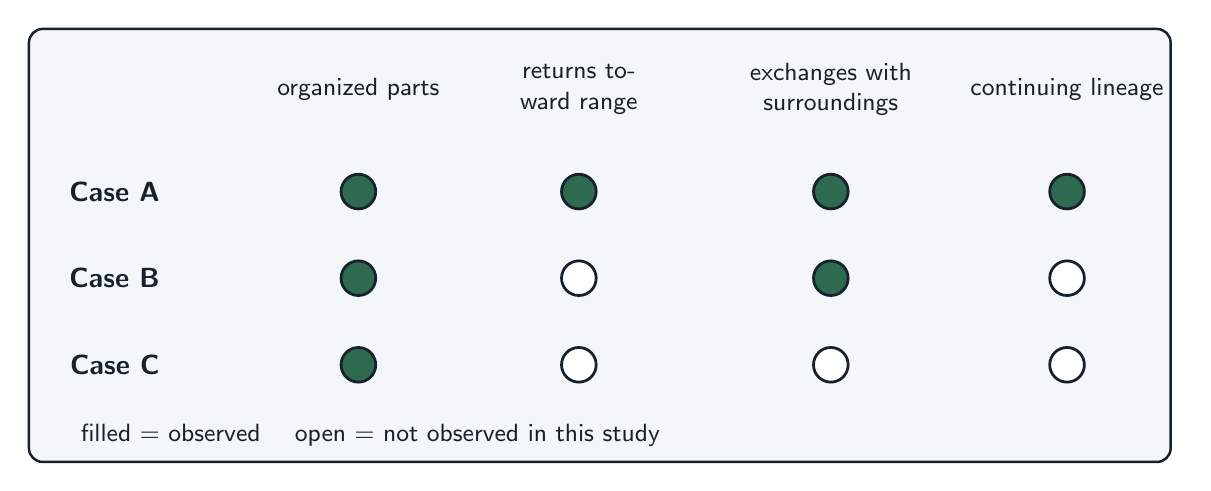
\begin{tikzpicture}[fc text, x=1cm, y=1cm]
  \node[fc panel, minimum width=145mm, minimum height=55mm, anchor=south west] at (0,0) {};
  \foreach \x/\t in {4.2/organized parts,7.0/returns toward range,10.2/exchanges with surroundings,13.2/continuing lineage} {
    \node[fc note, text width=27mm] at (\x,4.75) {\t};
  }
  \foreach \y/\lab in {3.45/Case A,2.35/Case B,1.25/Case C} {\node[fc label, anchor=east] at (1.8,\y) {\lab};}
  \foreach \x in {4.2,7.0,10.2,13.2} {\draw[draw=fcink, fill=fcgreen, line width=1pt] (\x,3.45) circle (2.2mm);}
  \foreach \x in {4.2,10.2} {\draw[draw=fcink, fill=fcgreen, line width=1pt] (\x,2.35) circle (2.2mm);}
  \foreach \x in {7.0,13.2} {\draw[draw=fcink, fill=white, line width=1pt] (\x,2.35) circle (2.2mm);}
  \draw[draw=fcink, fill=fcgreen, line width=1pt] (4.2,1.25) circle (2.2mm);
  \foreach \x in {7.0,10.2,13.2} {\draw[draw=fcink, fill=white, line width=1pt] (\x,1.25) circle (2.2mm);}
  \node[fc note, anchor=west] at (0.55,0.35) {filled = observed \quad open = not observed in this study};
\end{tikzpicture}
\end{document}
